\section{Интерфейс пользователя} \label{sub25} 

\subsection{Подготовка окружения пользователя} \label{subsub251}

Для того, что бы~IntelliJ~IDEA начала взаимодействовать с~GDSL модулем достаточно поместить модуль в~директорию проекта как показанно на~рис.~\ref{img:user-1}. Конкретное местоположение модуля не имеет значение, главное что бы оно было в области видимости среды (class path) IntelliJ~IDEA. При обнаружении GDSL-модуля, среда сразу же~включает его в~список обработчиков синтаксического анализа.

\begin{figure}[h!]
	\centering
	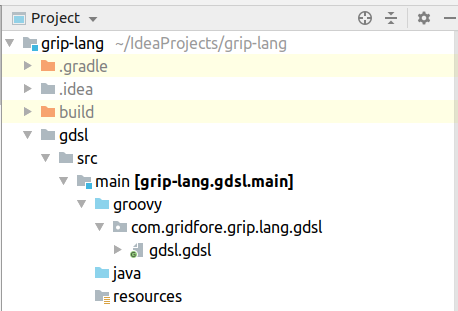
\includegraphics [scale=0.75] {user1}
	\caption{Интеграция GDSL модуля c~проектом пользователя}
	\label{img:user-1}
\end{figure}

Сам же~проект, согласно требованиям GRIP DSL, должен соблюдать структуру, которая представлена на~рис.~\ref{img:user-2}.

\begin{figure}[h!]
	\centering
	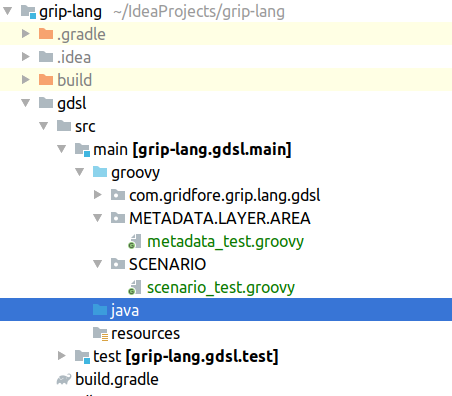
\includegraphics [scale=0.7] {user2}
	\caption{Структура проекта пользователя}
	\label{img:user-2}
\end{figure}

\subsection{Определение метаданных} \label{subsub252}

\textit{Метаданные}~--- набор выражений на~GRIP~DSL, который определяет имена и~типы полей, с~которыми будет работать пользователь.

В~пакете \texttt{metadata.layer.area}\footnote{Теринология Data Warehousing (хранилище данных). \textit{Layer}~---Data Source Layer (уровень источника данных), \textit{area}~--- Staging Area (область загрузки).} должен находиться один или несколько groovy скриптов, внутри которых определяются поля и~их~типы с~помощью GRIP~DSL, как показано на~рис.~\ref{img:user-3}

\begin{figure}[h!]
	\centering
	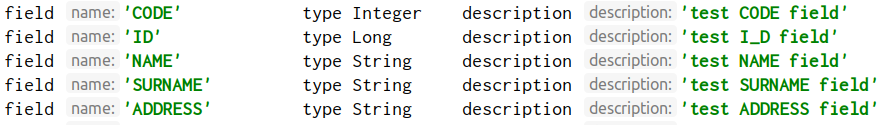
\includegraphics [scale=0.5] {user3}
	\caption{Определение метаданных}
	\label{img:user-3}
\end{figure}

\subsection{Поддержа метаданных в~сценариях исполнения} \label{subsub253}

\textit{Сценарий исполнения}~--- groovy скрипт, написанный на~диалекте GRIP~DSL, в~котором пользователь определяет интеграцию со~множеством хранилищ данных, их~обработку и~сохранение (\textit{Extract-Transform-Load, ETL}). Согласно GRIP~DSL, сценарий исполнения должен находиться в~пакете \texttt{scenario}.

В~процессе написания сценария исполнения пользователь использует метаданные, описанные в~пакете \texttt{metadata.layer.area} для более удобного и~гибкого описания ETL процесса. Поддержка метаданных в~сценарии исполнения представлена на~рис.~\ref{img:user-4}.

\begin{figure}[h!]
	\centering
	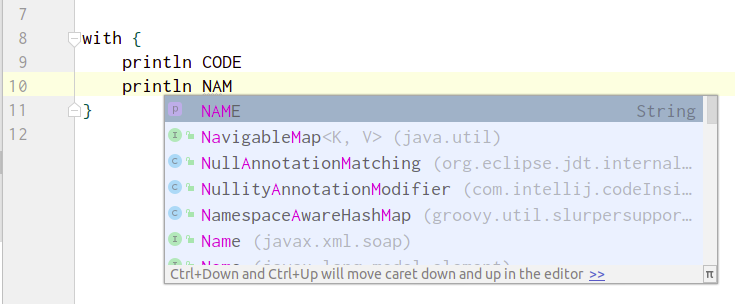
\includegraphics [scale=0.65] {user4}
	\caption{Подсветка синтаксиса и автодополнение метаданных}
	\label{img:user-4}
\end{figure}